\documentclass[aspectratio=169, 10pt]{beamer}
\usetheme{Hannover}
\usefonttheme{professionalfonts}

\definecolor{verdeuami}{RGB}{0,102,61}
\definecolor{eegaccent}{RGB}{0, 150, 136}
\definecolor{eeglight}{RGB}{224, 242, 241}

\setbeamercolor{frametitle}{bg=verdeuami, fg=white}
\setbeamercolor{title}{fg=white,bg=verdeuami}
\setbeamercolor{structure}{fg=verdeuami}
\setbeamercolor{block title}{bg=verdeuami, fg=white}
\setbeamercolor{block body}{bg=eeglight}
\setbeamercolor{alerted text}{fg=eegaccent}

\setbeamertemplate{navigation symbols}{}

\setbeamertemplate{footline}[frame number]



\usepackage{fontspec}
\setmainfont{TeX Gyre Termes}
  [BoldFont = TeX Gyre Termes Bold,
   ItalicFont = TeX Gyre Termes Italic]
\setsansfont{TeX Gyre Heros}
  [BoldFont = TeX Gyre Heros Bold,
   ItalicFont = TeX Gyre Heros Italic]
\setmonofont{TeX Gyre Cursor}

\usepackage{amsmath, amssymb}
\usepackage{pgf, graphicx}
\usepackage{booktabs}
\usepackage{hyperref}
\usepackage{microtype}
\usepackage{xcolor}
\usepackage{tikz}
\usepackage[spanish]{babel}
\usetikzlibrary{positioning, arrows.meta, shapes.geometric}
\usepackage{pdfpc-commands}

\pgfdeclareimage[height=0.8in]{logo}{shared/lini_original_landscape}

\title[qEEG]{Algunas exploraciones \\ en electorencefalografía cuantitativa}
\subtitle{De señal a biomarcador}
\author[OYS]{Oscar Yáñez Suárez\\\small oyanez@izt.uam.mx}
\institute[UAMI]{Ingeniería Eléctrica / UAM Iztapalapa}
\date{\today}
 \logo{
\includegraphics[height=0.8cm]{shared/lini_logo_original_small}} 

\begin{document}
	
	% slides/00_title.tex
\begin{frame}[plain]
  \titlegraphic{\pgfuseimage{logo}}
  \titlepage
\end{frame}

	% slides/01_outline.tex
\begin{frame}{Contenido}
  %\tableofcontents[hidesubsections]
  \begin{columns}[T]
  	\begin{column}{0.5\textwidth}
  		\tableofcontents[sections=1-5, subsectionstyle=hide/hide] 
  	\end{column}
  	\begin{column}{0.5\textwidth}
  		\tableofcontents[sections=6-, subsectionstyle=hide/hide] 
  	\end{column}
  \end{columns}
\end{frame}

	\section{Motivación y Contexto}
	\subsection{qEEG}
	\begin{frame}{Electroencefalografía}
    \begin{center}
		\inlineMovie[loop&autostart]{video/eeg.avi}{imagenes/eeg_snapshot.png}{width=0.8\linewidth}
		%\movie{
\includegraphics{../img/eeg_snapshot.png}}{../video/eeg.avi}
	\end{center}
\end{frame}

	% slides/02_motivation.tex


\begin{frame}{¿Por qué EEG cuantitativo?}
  \begin{columns}[T]
    \begin{column}{0.55\textwidth}
      \begin{itemize}
        \item El análisis \emph{clásico} del EEG parte de la \alert{inspección visual} — subjetiva, lenta, dependiente del experto
        \item[]
        \item El qEEG extrae \alert{rasgos numéricos objetivos y reproducibles} a partir de las señales crudas
        \item[]
        \item Posibilita los estudios poblacionales de gran escala, las interfaces cerebro-computadora en tiempo real, y el descubrimiento de biomarcadores
      \end{itemize}
    \end{column}
    \begin{column}{0.42\textwidth}
    	Confluencia de:
			\begin{itemize}
				\item Sistemas de alta densidad (256+ electrodos)
				\item Pipelines extendibles de software libre (MNE, BCI2000)
				\item Herramientas modernas de aprendizaje maquinal
			\end{itemize}
      \vspace{0.5em}
      \begin{block}{Referencias clave}
        \small
        Nuwer \textit{et al.}\ (1998) establecen estándares básicos de qEEG \cite{Nuwer1999} \\
        \vspace{5pt}
        Makeig \textit{et al.}\ (2004) consolidan el análisis de la dinámica cerebral \cite{Makeig2004}.
      \end{block}
    \end{column}
  \end{columns}
\end{frame}

	\subsection{EEG 101}
	% slides/03_eeg_primer.tex
\begin{frame}{EEG 101}
  \begin{columns}[T]
    \begin{column}{0.50\textwidth}
      \textbf{Generación}
      \begin{itemize}
        \item Potenciales post-sinápticos en las dendritas apicales de neuronas piramidales
        \item \emph{¡También potenciales de acción!}
        \item Conducción por el volumen de LCR/cráneo/piel cabelluda
      \end{itemize}
      \vspace{0.8em}
      \textbf{Interpretación \emph{clásica} en bandas}
        \small
        \begin{tabular}{lll}
          \toprule
          Banda & Rango (Hz) & Correlato cognitivo \\
          \midrule
          $\delta$ & 0.5--4   & Sueño profundo, patología \\
          $\theta$ & 4--8     & Memoria, somnolencia \\
          $\alpha$ & 8--13    & Vigilia \\
          $\beta$  & 13--30   & Cognición activa \\
          $\gamma$ & 30--100+ & Fijación, percepción \\
          \bottomrule
        \end{tabular}
    \end{column}
    \begin{column}{0.5\textwidth}
    	\begin{block}{Referencia clave}
    		\small
    		Fernandez-Ruiz \textit{et al.} (2023) asocian las oscilaciones gamma con la operación de circuitos neuronales \cite{Fernandez-Ruiz2023}.
    	\end{block}
    \end{column}
  \end{columns}
\end{frame}

	% slides/03_eeg_primer.tex
\begin{frame}{EEG 101}
  \begin{columns}[T]
    \begin{column}{0.50\textwidth}
      \textbf{Artefactos de medición}
\begin{itemize}
	\item \textit{Ocular}: parpadeos (EOG), movimientos sacádicos
	\item \textit{Muscular}: EMG ($>$30 Hz)
	\item \textit{Cardiaco}: ECG, BCG
	\item \textit{Entorno}: ruido de linea, deriva electródica
\end{itemize}
    \end{column}
    \begin{column}{0.5\textwidth}
      \vspace{0.3em}
      \begin{block}{Nota práctica}
        \small La elección de referencia (CAR, mastoides ligados, REST) impacta críticamente los resultados espectrales y de conectividad \cite{Yao2001}.
      \end{block}
    \end{column}
  \end{columns}
\end{frame}

	% slides/04_history.tex
\begin{frame}{Línea del tiempo de la qEEG}
  \begin{center}
  \begin{tikzpicture}[
      node distance = 0.55cm and 0.1cm,
      every node/.style = {font=\small},
      milestone/.style = {draw=verdeuami, fill=eeglight, rounded corners=3pt,
                          text width=2.5cm, align=center, inner sep=4pt},
      arr/.style = {-Stealth, thick, color=verdeuami}
    ]
    \node[milestone] (berger) {1929\\Berger\\Primer EEG};
    \node[milestone, right=of berger] (fft)    {1965\\Cooley \& Tukey\\Algoritmo FFT};
    \node[milestone, right=of fft]    (dipole) {1980s\\Ajuste de dipolos\\BESA};
    \node[milestone, right=of dipole] (loreta) {1994\\Pascual-Marqui\\LORETA};
    \node[milestone, below=0.6cm of loreta] (ica)    {1996\\Bell \& Sejnowski\\ICA para EEG};
    \node[milestone, below=0.6cm of ica]  (conn) {2000s\\Conectividad\\PLV, PDC};
    \node[milestone, left=of conn]  (hd)  {2010s\\HD-EEG\\sLORETA};
    \node[milestone, left=of hd]    (dl)  {2018+\\Aprendizaje\\EEGNet, BENDR};
    \node[milestone, left=of dl]    (fm)  {2023+\\LLMs\\LaBraM};
    \draw[arr] (berger) -- (fft);
    \draw[arr] (fft)    -- (dipole);
    \draw[arr] (dipole) -- (loreta);
    \draw[arr] (loreta) -- (ica);
    \draw[arr] (ica)    -- (conn);
    \draw[arr] (conn)   -- (hd);
    \draw[arr] (hd)     -- (dl);
    \draw[arr] (dl)     -- (fm);
  \end{tikzpicture}
  \end{center}
  \vspace{0.2em}
  \small Referencias: \cite{Berger1929,CooleyTukey1965,PascualMarqui1994,BellSejnowski1995,LeVanQuyen2001}
\end{frame}

	\begin{frame}{Hans Berger, 1929}
    \begin{center}
    	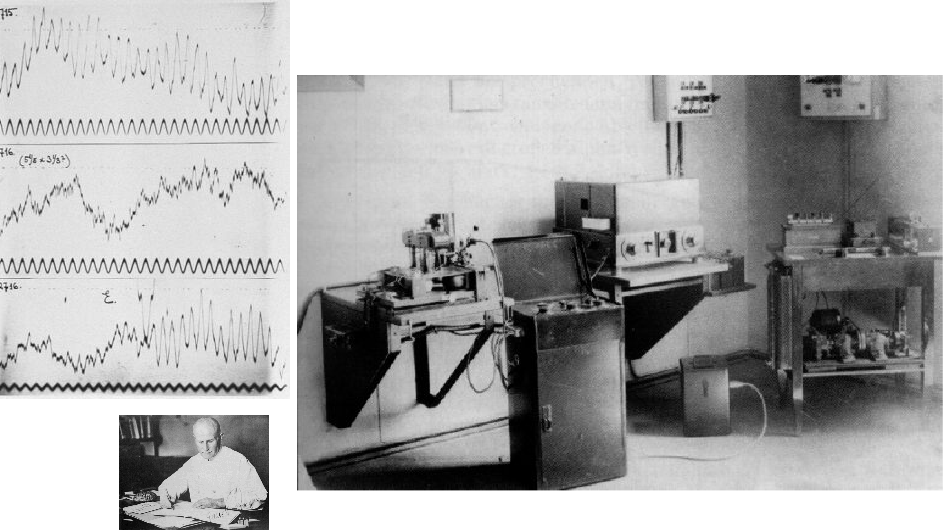
\includegraphics[width=\textwidth]{imagenes/berger_collage.png}
	\end{center}
\end{frame}

	% slides/05_preprocessing.tex


\begin{frame}{Flujo de trabajo de preprocesamiento en qEEG}
  \begin{columns}[T]
    \begin{column}{0.52\textwidth}
      \textbf{Procesos comunes}
      \begin{enumerate}
        \item Cambio de referencia (CAR / REST)
        \item Filtrado pasa/rechaza banda
        \item Segmentación basada en tiempo o en marcas
        \item Rechazo/interpolación de épocas 
        \item Artifact subspace reconstruction (ASR) \cite{Mullen2015}
        \item Descomposición y clasificación de componentes ICA (ICLabel) \cite{PionTonachini2019}
      \end{enumerate}
    \end{column}
    \begin{column}{0.45\textwidth}
      \begin{alertblock}{Matriz de confusión ICLabel}
      	\begin{center}
        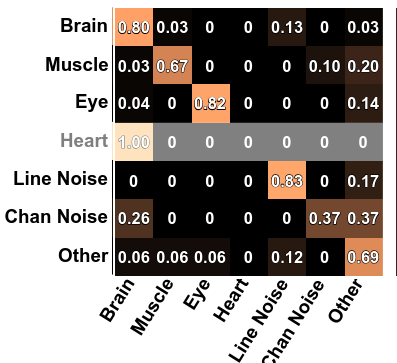
\includegraphics[width=0.7\textwidth]{imagenes/iclabel.png}
        \end{center}
      \end{alertblock}
    \end{column}
  \end{columns}
\end{frame}

	\begin{frame}{Reconstrucción post-ICLabel}
	\begin{center}
		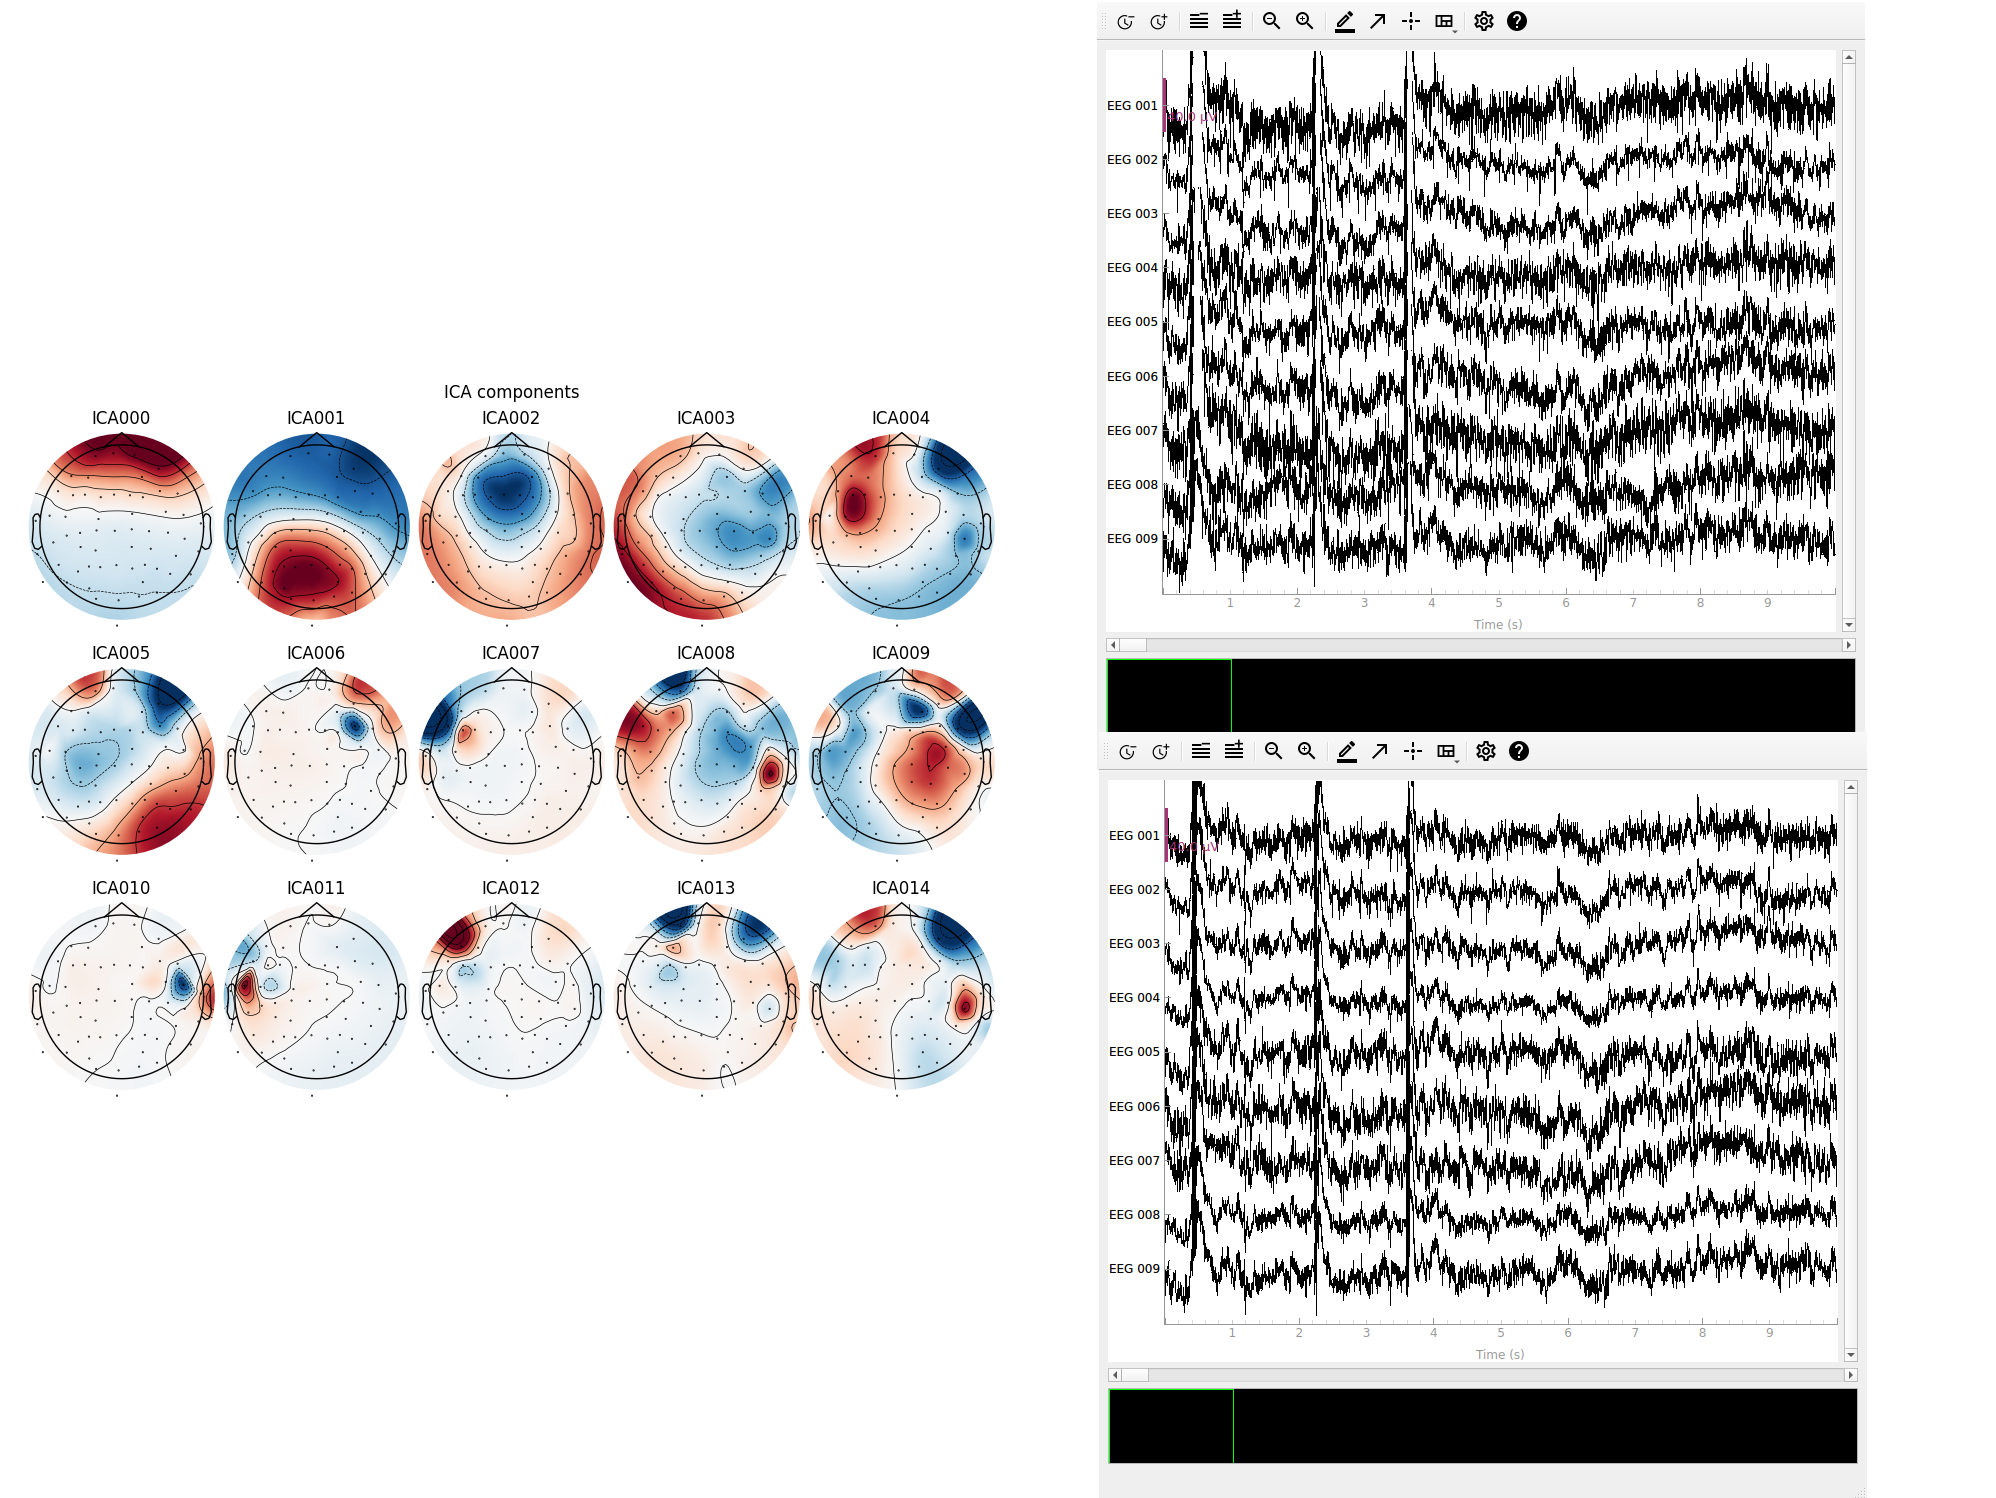
\includegraphics[width=0.8\textwidth]{imagenes/iclabel_plots.png}
	\end{center}
\end{frame}
	\section{Análisis del EEG}
	\subsection{Espectral}
	% slides/06_spectral.tex


\begin{frame}{Más allá de la TDF}
  \begin{columns}[T]
    \begin{column}{0.50\textwidth}
      \textbf{Descomposiciones ortogonales}
      \begin{itemize}
        \item CSP - Filtrado basado en componentes principales 
      \end{itemize}
      \vspace{0.4em}
      \textbf{Descomposiciones redundantes}
      \begin{itemize}
        \item Descomposición empírica en modos (EMD)
      \end{itemize}
    \end{column}
    \begin{column}{0.47\textwidth}
      \textbf{Representaciones tiempo-frecuencia}
      \begin{itemize}
        \item STFT / espectrograma
        \item BPts  (Bojorges, Pardo, Yáñez) \cite{Pardo2025}
        \item Wavelets \cite{Tallon-Baudry1997, Moca2021}
      \end{itemize}
      \vspace{0.3em}
    \end{column}
  \end{columns}
\end{frame}

	\subsection{Conectividad funcional}
	% slides/07_connectivity.tex


\begin{frame}{Functional \& Effective Connectivity}
  \begin{columns}[T]
    \begin{column}{0.50\textwidth}
      \textbf{Undirected (functional) measures}
      \begin{itemize}
        \item \textbf{Coherence}: spectral correlation — volume-conduction sensitive
        \item \textbf{PLV} (phase-locking value): phase synchrony, ignores
          amplitude \cite{LeVanQuyen2001}
        \item \textbf{PLI / wPLI}: imaginary component only $\Rightarrow$ robust
          to zero-lag artefacts \cite{Vinck2011}
        \item \textbf{AEC} (amplitude envelope correlation): slow fluctuations
          in broadband power
      \end{itemize}
    \end{column}
    \begin{column}{0.47\textwidth}
      \textbf{Directed (effective) measures}
      \begin{itemize}
        \item \textbf{Granger causality} / MVAR models \cite{Granger1969}
        \item \textbf{DTF / PDC}: partial directed coherence in frequency domain
        \item \textbf{Transfer entropy}: model-free, information-theoretic
        \item \textbf{DCM}: Bayesian, mechanistic \cite{Friston2003}
      \end{itemize}
      \vspace{0.3em}
      \begin{alertblock}{Phase--amplitude coupling (PAC)}
        \small Coupling between $\theta$ phase and $\gamma$ amplitude
        tracks working memory load \cite{Canolty2006}.
      \end{alertblock}
    \end{column}
  \end{columns}
\end{frame}

	\subsection{Tomografía eléctrica}
	% slides/08_source.tex


\begin{frame}{Solving the EEG Inverse Problem}
  \begin{columns}[T]
    \begin{column}{0.50\textwidth}
      \textbf{The inverse problem is ill-posed}
      \begin{itemize}
        \item Infinitely many source configurations can produce the same scalp topography
        \item Regularisation and anatomical priors are essential
      \end{itemize}
      \vspace{0.4em}
      \textbf{LORETA family} \cite{PascualMarqui1994}
      \begin{itemize}
        \item \textbf{LORETA}: Laplacian smoothness prior
        \item \textbf{sLORETA}: zero localisation error for single dipoles
        \item \textbf{eLORETA}: exact, standardised; gold standard for resting-state
      \end{itemize}
    \end{column}
    \begin{column}{0.47\textwidth}
      \textbf{Beamforming}
      \begin{itemize}
        \item \textbf{LCMV}: scalar/vector; optimal for ERPs
        \item \textbf{DICS}: frequency-domain; ideal for oscillatory sources \cite{Gross2001}
        \item Requires accurate covariance — sensitive to artifact residuals
      \end{itemize}
      \vspace{0.3em}
      \textbf{MRI-constrained methods}
      \begin{itemize}
        \item Individual head models (BEM, FEM)
        \item Cortical surface constraint (FreeSurfer parcellations)
        \item Combined EEG-fMRI asymptotic approaches
      \end{itemize}
    \end{column}
  \end{columns}
\end{frame}

	\subsection{Interfaz cerebro computadora}
	% slides/09_ml.tex


\begin{frame}{Machine \& Deep Learning on EEG}
  \begin{columns}[T]
    \begin{column}{0.50\textwidth}
      \textbf{Classical feature engineering}
      \begin{itemize}
        \item Band power, spectral entropy, Hjorth parameters
        \item AR coefficients, coherence matrices
        \item Riemannian geometry of covariance matrices \cite{Barachant2012}
        \item CSP + LDA pipeline (motor imagery BCI)
      \end{itemize}
      \vspace{0.3em}
      \textbf{Shallow classifiers}
      \begin{itemize}
        \item SVM, Random Forest, LDA
        \item XGBoost on spectral features
        \item Transfer learning via Euclidean alignment
      \end{itemize}
    \end{column}
    \begin{column}{0.47\textwidth}
      \textbf{Deep learning architectures}
      \begin{itemize}
        \item \textbf{EEGNet}: compact depthwise CNN; cross-task
          generalisation \cite{Lawhern2018}
        \item \textbf{ShallowConvNet / DeepConvNet} \cite{Schirrmeister2017}
        \item \textbf{EEG-Conformer}: self-attention over channels \& time \cite{Song2022}
        \item \textbf{BENDR}: contrastive self-supervised pretraining \cite{Kostas2022}
        \item \textbf{LaBraM}: foundation model, cross-dataset pretraining \cite{Jiang2024}
      \end{itemize}
      \vspace{0.2em}
      \begin{block}{Open challenge}
        \small Cross-subject and cross-device generalisation
        remain unsolved without domain adaptation.
      \end{block}
    \end{column}
  \end{columns}
\end{frame}

	% slides/10_microstates.tex

\begin{frame}{EEG Microstates \& Nonlinear Complexity}
  \begin{columns}[T]
    \begin{column}{0.52\textwidth}
      \textbf{EEG Microstates}
      \begin{itemize}
        \item Global scalp topography quasi-stable for $\sim$60--120 ms
        \item Canonical 4--7 classes (A--G) via k-means / AAHC \cite{Michel2018}
        \item Sequence statistics: duration, occurrence rate, transition matrix
        \item Classes A--D map to dorsal attention, visual, somatomotor,
          DMN networks \cite{Britz2010}
        \item Altered in schizophrenia, depression, Alzheimer's disease
      \end{itemize}
    \end{column}
    \begin{column}{0.45\textwidth}
      \textbf{Nonlinear complexity measures}
      \begin{itemize}
        \item \textbf{SampEn}: regularity of temporal patterns;
          reduced in coma \cite{Richman2000}
        \item \textbf{Lempel--Ziv}: compressibility of binarised signal
        \item \textbf{DFA}: long-range temporal correlations
        \item \textbf{Lyapunov exponent}: phase-space divergence
      \end{itemize}
      \vspace{0.2em}
      \begin{alertblock}{Brain criticality}
        \small Healthy resting-state EEG sits near a critical point;
        complexity shifts towards subcriticality in anaesthesia
        and DOC \cite{Tagliazucchi2012}.
      \end{alertblock}
    \end{column}
  \end{columns}
\end{frame}

	\section{Aplicaciones clínicas}
	% slides/11_clinical_epilepsy_sleep.tex


\begin{frame}{Clinical Applications I: Epilepsy \& Sleep}
  \begin{columns}[T]
    \begin{column}{0.50\textwidth}
      \textbf{Epilepsy}
      \begin{itemize}
        \item \textbf{Automated seizure detection}: CNN/LSTM on raw iEEG
          reaches $>$95\% sensitivity \cite{Subasi2005}
        \item \textbf{Seizure prediction}: phase-space features, 30--60 min
          pre-ictal window
        \item \textbf{Spike detection}: template matching, iEEG atlas
        \item HFOs (high-frequency oscillations) as epileptogenic zone markers
      \end{itemize}
    \end{column}
    \begin{column}{0.47\textwidth}
      \textbf{Sleep staging}
      \begin{itemize}
        \item AASM rules (W/N1/N2/N3/REM) automatable at $\sim$85\% epoch accuracy
        \item \textbf{U-Sleep}: universal model across PSG montages \cite{Perslev2021}
        \item Spindle \& K-complex detection: matched filters + neural networks
        \item HRV--EEG coupling for sleep quality metrics
      \end{itemize}
      \vspace{0.3em}
      \begin{block}{Key toolboxes}
        \small EEGLAB, MNE-Python, FieldTrip, Brainstorm, YASA (sleep)
      \end{block}
    \end{column}
  \end{columns}
\end{frame}

	% slides/12_clinical_psychiatry.tex
\begin{frame}{Aplicaciones clínicas II: psiquiatría}
  \begin{columns}[T]
    \begin{column}{0.50\textwidth}
      \textbf{Biomarcadores psiquiátricos}
      \begin{itemize}
        \item Depresión: la asimetría $\alpha$ frontal (F4-F3)
          predice la respuesta al tratamiento \cite{Harmon-Jones2003}
        \item Esquizofrenia: Reducción de la amplitud de MMN; baja potencia $\gamma$
        \item TDAH: tasa $\theta/\beta$ elevada (controversial)
        \item Alzheimer's: descenso de la frecuencia pico en la banda $\alpha$,
          pérdida de coherencia
         \item Neurofeedback (¿?)
      \end{itemize}
    \end{column}
    \begin{column}{0.47\textwidth}
    	
\includegraphics[width=\textwidth]{imagenes/neuro_psi.png}
    \end{column}
  \end{columns}
\end{frame}

	\section{Limitaciones y perspectivas}
	% slides/13_limitations.tex

\begin{frame}{Problemas abiertos}
  \begin{columns}[T]
    \begin{column}{0.50\textwidth}
      \textbf{Retos metodológicos}
      \begin{itemize}
        \item Resolución espacial
        \item No hay una referencia neutra real
        \item Los supuestos de estacionaridad regularmente no se cumplen
        \item Muestras pequeñas
      \end{itemize}
    \end{column}
    \begin{column}{0.47\textwidth}
      \textbf{En el aprendizaje maquinal}
      \begin{itemize}
        \item Interpretabilidad
        \item Generalización: gran variabilidad inter-sujeto
        \item Transferencia: diferentes setups por laboratorio
        \item Nuestras pequeñas (¿privacidad?)
      \end{itemize}
      \vspace{0.3em}
      \begin{block}{Reproducibilidad}
        \small Variosl biomarcadores basados en qEEG (razón $\theta/\beta$, asimetría $\alpha$, BIS) han fallado pruebas de reproducibilidad a gran escala.
      \end{block}
    \end{column}
  \end{columns}
\end{frame}

	% slides/14_conclusions.tex
\begin{frame}{Conclusiones}
  \begin{columns}[T]
    \begin{column}{0.55\textwidth}
      \textbf{Resumen}
      \begin{itemize}
        \item qEEG ha madurado en una multidisciplina
        \item La corrección de artefactos es casi un problema resuelto
        \item El conectoma humano sigue siendo un enorme problema
        \item Los grandes modelos de EEG (LLMs) anuncian un próximo cambio paradigmático en la disciplina
      \end{itemize}
    \end{column}
    \begin{column}{0.42\textwidth}
      \textbf{En la frontera ...}
      \begin{itemize}
        \item Multimodalidad:\\EEG + fMRI + fNIRS
        \item Ambulatorio:\\Electrodos secos, optodos
        \item Causalidad:\\observar las perturbaciones por TMS, TDCS
        \item LLMs:\\decodificar tareas/estados mentales
      \end{itemize}
    \end{column}
  \end{columns}
  \vspace{0.5em}
  \begin{center}
    \alert{\textit{``The brain is wider than the sky ....'' \\ Emily Dickinson}}
  \end{center}
\end{frame}

	% slides/15_references.tex
\section*{Referencias}

\begin{frame}[allowframebreaks]{Referencias}
  \footnotesize
  \begin{thebibliography}{99}

    \bibitem{Berger1929}
    H.~Berger, ``Über das Elektrenkephalogramm des Menschen,''
    \textit{Arch. Psychiatr. Nervenkr.}, vol.~87, pp.~527--570, 1929.

    \bibitem{CooleyTukey1965}
    J.~W.~Cooley and J.~W.~Tukey, ``An algorithm for the machine calculation of complex Fourier series,''
    \textit{Math. Comput.}, vol.~19, pp.~297--301, 1965.

    \bibitem{BellSejnowski1995}
    A.~J.~Bell and T.~J.~Sejnowski, ``An information-maximization approach to blind separation,''
    \textit{Neural Comput.}, vol.~7, no.~6, pp.~1129--1159, 1995.

    \bibitem{PascualMarqui1994}
    R.~D.~Pascual-Marqui, C.~M.~Michel, and D.~Lehmann,
    ``Low resolution electromagnetic tomography,''
    \textit{Int. J. Psychophysiol.}, vol.~18, no.~1, pp.~49--65, 1994.

    \bibitem{Nuwer1999}
    M.~R.~Nuwer \textit{et al.}, ``IFCN standards for digital recording of clinical EEG,''
    \textit{Electroencephalogr. Clin. Neurophysiol.}, vol.~106, pp.~259--261, 1998.

    \bibitem{Makeig2004}
    S.~Makeig \textit{et al.}, ``Mining event-related brain dynamics,''
    \textit{Trends Cogn. Sci.}, vol.~8, no.~5, pp.~204--210, 2004.

    \bibitem{Yao2001}
    D.~Yao, ``A method to standardize a reference of scalp EEG recordings to a point at infinity,''
    \textit{Physiol. Meas.}, vol.~22, no.~4, pp.~693--711, 2001.
    
    \bibitem{Fernandez-Ruiz2023}
    A.~Fernandez-Ruiz \textit{et al.} ``Over and above frequency: Gamma oscillations as units of neural circuit operations,'' \textit{Neuron}, vol.~111, no.~7, pp.~936--953, 2023.
    
    \bibitem{Pardo2025}
    M.~Pardo-Rodriguez \textit{et al.} ``Conscious breathing enhances bidirectional cortical-autonomic modulation: dynamics of EEG band power and heart rate variability,'' \textit{Front. Syst. Neurosci.,}, vol.~19, pp.~1--16, 2025.

    \bibitem{Thomson1982}
    D.~J.~Thomson, ``Spectrum estimation and harmonic analysis,''
    \textit{Proc. IEEE}, vol.~70, no.~9, pp.~1055--1096, 1982.

    \bibitem{HuangEtAl1998}
    N.~E.~Huang \textit{et al.}, ``The empirical mode decomposition and the Hilbert spectrum,''
    \textit{Proc. R. Soc. Lond. A}, vol.~454, pp.~903--995, 1998.

    \bibitem{Tallon-Baudry1997}
    C.~Tallon-Baudry \textit{et al.}, ``Oscillatory gamma-band (30--70 Hz) activity
    induced by a visual search task in humans,''
    \textit{J. Neurosci.}, vol.~17, no.~2, pp.~722--734, 1997.

    \bibitem{Moca2021}
    V.~V.~Moca \textit{et al.}, ``Time-frequency super-resolution with superlets,''
    \textit{Nat. Commun.}, vol.~12, p.~337, 2021.

    \bibitem{LeVanQuyen2001}
    M.~Le~Van~Quyen \textit{et al.}, ``Comparison of Hilbert transform and wavelet methods
    for the analysis of neuronal synchrony,''
    \textit{J. Neurosci. Methods}, vol.~111, no.~2, pp.~83--98, 2001.

    \bibitem{Vinck2011}
    M.~Vinck \textit{et al.}, ``An improved index of phase-synchronization for
    electrophysiological data,''
    \textit{NeuroImage}, vol.~55, no.~4, pp.~1548--1565, 2011.

    \bibitem{Granger1969}
    C.~W.~J.~Granger, ``Investigating causal relations by econometric models
    and cross-spectral methods,''
    \textit{Econometrica}, vol.~37, no.~3, pp.~424--438, 1969.

    \bibitem{Friston2003}
    K.~J.~Friston \textit{et al.}, ``Dynamic causal modelling,''
    \textit{NeuroImage}, vol.~19, no.~4, pp.~1273--1302, 2003.

    \bibitem{Canolty2006}
    R.~T.~Canolty \textit{et al.}, ``High gamma power is phase-locked
    to theta oscillations in human neocortex,''
    \textit{Science}, vol.~313, pp.~1626--1628, 2006.

    \bibitem{Gross2001}
    J.~Gross \textit{et al.}, ``Dynamic imaging of coherent sources,''
    \textit{Proc. Natl. Acad. Sci.}, vol.~98, no.~2, pp.~694--699, 2001.

    \bibitem{Mullen2015}
    T.~R.~Mullen \textit{et al.}, ``Real-time neuroimaging and cognitive monitoring
    using wearable dry EEG,''
    \textit{IEEE Trans. Neural Syst. Rehabil. Eng.}, vol.~23, no.~6, pp.~843--848, 2015.

    \bibitem{PionTonachini2019}
    L.~Pion-Tonachini \textit{et al.}, ``ICLabel: An automated electroencephalographic
    independent component classifier,''
    \textit{NeuroImage}, vol.~198, pp.~181--197, 2019.

    \bibitem{Ablin2018}
    P.~Ablin \textit{et al.}, ``Faster independent component analysis by preconditioning
    with Hessian approximations,''
    \textit{IEEE Trans. Signal Process.}, vol.~66, no.~15, pp.~4040--4049, 2018.

    \bibitem{Palmer2011}
    J.~A.~Palmer \textit{et al.}, ``Newton method for the ICA mixture model,''
    \textit{Proc. ICASSP}, 2008.

    \bibitem{Barachant2012}
    A.~Barachant \textit{et al.}, ``Multiclass brain--computer interface classification
    by Riemannian geometry,''
    \textit{IEEE Trans. Biomed. Eng.}, vol.~59, no.~4, pp.~920--928, 2012.

    \bibitem{Lawhern2018}
    V.~J.~Lawhern \textit{et al.}, ``EEGNet: a compact convolutional neural network
    for EEG-based brain--computer interfaces,''
    \textit{J. Neural Eng.}, vol.~15, no.~5, p.~056013, 2018.

    \bibitem{Schirrmeister2017}
    R.~T.~Schirrmeister \textit{et al.}, ``Deep learning with convolutional neural networks
    for EEG decoding and visualization,''
    \textit{Hum. Brain Mapp.}, vol.~38, no.~11, pp.~5391--5420, 2017.

    \bibitem{Song2022}
    Y.~Song \textit{et al.}, ``EEG conformer: Convolutional transformer for EEG
    signal decoding and visualization,''
    \textit{IEEE Trans. Neural Syst. Rehabil. Eng.}, vol.~31, pp.~710--719, 2022.

    \bibitem{Kostas2022}
    D.~Kostas \textit{et al.}, ``BENDR: using transformers and a contrastive
    self-supervised learning task to learn from massive amounts of EEG data,''
    \textit{Front. Hum. Neurosci.}, vol.~15, p.~653659, 2021.

    \bibitem{Jiang2024}
    W.~Jiang \textit{et al.}, ``Large brain model for learning generic representations
    with tremendous EEG data in BCI,''
    \textit{ICLR}, 2024.

    \bibitem{Michel2018}
    C.~M.~Michel and T.~Koenig, ``EEG microstates as a tool for studying the temporal
    dynamics of whole-brain neuronal networks,''
    \textit{NeuroImage}, vol.~180, pp.~577--593, 2018.

    \bibitem{Britz2010}
    J.~Britz \textit{et al.}, ``BOLD correlates of EEG topography reveal rapid
    resting-state network dynamics,''
    \textit{NeuroImage}, vol.~52, no.~4, pp.~1162--1170, 2010.

    \bibitem{Richman2000}
    J.~S.~Richman and J.~R.~Moorman, ``Physiological time-series analysis using
    approximate entropy and sample entropy,''
    \textit{Am. J. Physiol.}, vol.~278, no.~6, pp.~H2039--H2049, 2000.

    \bibitem{Tagliazucchi2012}
    E.~Tagliazucchi \textit{et al.}, ``Criticality in large-scale brain fMRI dynamics,''
    \textit{Front. Physiol.}, vol.~3, p.~15, 2012.

    \bibitem{Subasi2005}
    A.~Subasi, ``Automatic recognition of alertness level from EEG,''
    \textit{Expert Syst. Appl.}, vol.~28, no.~4, pp.~701--711, 2005.

    \bibitem{Perslev2021}
    M.~Perslev \textit{et al.}, ``U-Sleep: resilient high-frequency sleep staging,''
    \textit{npj Digit. Med.}, vol.~4, p.~72, 2021.

    \bibitem{Harmon-Jones2003}
    E.~Harmon-Jones and J.~J.~B.~Allen,
    ``Behavioral activation sensitivity and resting frontal EEG asymmetry,''
    \textit{J. Abnorm. Psychol.}, vol.~106, no.~1, pp.~159--163, 1997.

    \bibitem{Casali2013}
    A.~G.~Casali \textit{et al.}, ``A theoretically based index of consciousness
    independent of sensory processing and behavior,''
    \textit{Sci. Transl. Med.}, vol.~5, no.~198, p.~198ra105, 2013.

    \bibitem{Sitaram2017}
    R.~Sitaram \textit{et al.}, ``Closed-loop brain training: the science of neurofeedback,''
    \textit{Nat. Rev. Neurosci.}, vol.~18, no.~2, pp.~86--100, 2017.

  \end{thebibliography}
\end{frame}

	% slides/16_goodbye.tex
\begin{frame}[plain]
  \begin{center}
    \vspace{1.5cm}
    {\Large \textbf{¡Gracias por su atención!}}\\[1em]
    {\large ¿Preguntas?}\\[2em]
    \textit{oyanez@izt.uam.mx}\\[0.5em]
    \begin{center}
    	
\includegraphics[width=0.25\textwidth]{shared/github_repo_qr.png}
    \end{center}
     \small Archivos de la presentación en:\\
      \texttt{https://github.com/oscarys/2026\_PIB}
  \end{center}
\end{frame}

	
\end{document}



%\documentclass{beamer}
%\mode<presentation>
%{
%  \usetheme{Warsaw}
%  %\usetheme[compress]{Dresden}
%  \setbeamercovered{invisible}
%}
%
%\usepackage{amsmath,amssymb,array}
%\usepackage[spanish]{babel}
%\usepackage{fontspec}
%%\usepackage[utf8x]{inputenc}
%\usepackage{pgf,graphicx,overpic,subfigure}
%
%\usepackage{pdfpc-commands}
%
%\title[qEEG-Conectividad]{Algunas exploraciones \\ en electorencefalografía cuantitativa\\ {\small Seminario del Posgrado de Ingeniería Biomédica, 26-I}}
%\author[Seminario PIB]{Laboratorio de Neuroimagenología - LINI}
%\institute[]{ Oscar Yáñez Suárez \\ Laboratorio de Neuroimagenología \\ UAM Iztapalapa \\ \texttt{oyanez@izt.uam.mx}}
%\date[]{}
%\subject{}
%
%\pgfdeclareimage[height=0.6in]{logo}{imagenes/inr-lini}
%\usecolortheme[rgb={0.0,0.4,0.2}]{structure} % Colores UAMI
%\definecolor{vuami}{rgb}{0.0,0.4,0.2}
%
%\begin{document}
%	
%	\include{portada}
%	\include{contenido}
%	\section{Introducción}
%		\subsection{Electrodiagnóstico y qEEG}
%		\include{colaboracion_inr_uam}
%		\include{eeg_scroll}
%		\include{graficas_inr_uami}
%	\section{Teoría de gráficas}
%		\subsection{Definiciones}
%		\include{tdg_definiciones}
%		\subsection{Ejemplos}
%		\include{grafica_republica_mexicana}
%		\include{grafica_1020}
%		\include{ejemplo_tdg_klimesch}
%		\subsection{Propiedades}
%		\include{tdg_medidas_nodo}
%		\include{tdg_medidas_grafica_no_pesada}
%	\section{Conectividad funcional}
%		\subsection{Medidas de conectividad}
%		\include{medidas_conectividad}
%		\subsection{Coherencia espectral}
%		\include{coherencia_espectral}
%		\include{graficas_de_conectividad_no_direcccional}
%		\include{graficas_de_conectividad_direcccional}
%		\subsection{Cuantificación de la conectividad}
%		\include{cuantificacion_redes_umbralizacion}
%		\include{cuantificacion_redes_promedio_coherencia}
%		\include{cuantificacion_redes_curso_temporal}
%	\section{Conclusiones}
%		\include{conclusiones}	
%		
%\end{document}